\documentclass[a4paper,titlepage]{article}
\usepackage[utf8]{inputenc}
\usepackage{fullpage}
\usepackage{indentfirst}
\usepackage[per-mode=symbol]{siunitx}
\usepackage{listings}
\usepackage{graphicx}
\usepackage{color}
\usepackage{amsmath}
\usepackage{mathtools}
\usepackage{array}
\usepackage[hidelinks]{hyperref}
\usepackage[format=plain,font=it]{caption}
\usepackage{subcaption}
\usepackage{standalone}
\usepackage[nottoc]{tocbibind}
\usepackage[noabbrev,capitalize,nameinlink]{cleveref}
\usepackage{listings}
\usepackage{xspace}
\usepackage{tikz}
\usepackage{circuitikz}
\usepackage{titlesec}
\usepackage[cache=false]{minted}
\usepackage{booktabs}
\usepackage{csvsimple}
\newcommand{\MATLAB}{\textsc{Matlab}\xspace}
\usepackage{siunitx}
\usepackage[super]{nth}
\usepackage[titletoc]{appendix}

% Custom commands
\newcommand\numberthis{\addtocounter{equation}{1}\tag{\theequation}}
\newcommand{\code}[1]{\texttt{#1}}
\newcolumntype{P}[1]{>{\centering\arraybackslash}p{#1}}

\tikzstyle{my help lines}=[gray,thick,dashed]

\setminted{linenos,breaklines,fontsize=auto}

%\titleformat*{\section}{\normalsize\bfseries}
%\titleformat*{\subsection}{\small\bfseries}
\renewcommand{\thesubsection}{\thesection.\alph{subsection}}
\providecommand*{\listingautorefname}{Listing}
\newcommand*{\Appendixautorefname}{Appendix}

%opening
\title{\textbf{ECSE 543: Numerical Methods} \\ Assignment 3 Report}
\author{Wenjie Wei \\ 260685967}
\date{\today}

\begin{document}
	\sloppy
	\maketitle
	
	\tableofcontents
	\newpage
	
	\twocolumn
	\section*{Introduction}
		This assignment explored the use of linear interpolations and other mathematical methods. The programs are programmed and compiled using Python 3.6, and the plots are generated using package matlibplot. Listing \ref{lst:poly} shows the implementations of polynomials including their possible maneuvers. The object classes included in this file will be used for the interpolations. 
		
	\section{Linear Interpolation of BH Points}
		\subsection{Lagrange Full Domain Interpolation of First Six-Point Set}
			Listing \ref{lst:interp} shows the implementation of various interpolation methods. For the first six points, the Lagrange interpolation shows an interpolated polynomial
			\begin{align*}
				B(h) = &9.275\times 10^{-12}h^5 - 5.951\times 10^{-9}h^4 \\
					   &+ 1.469\times 10^{-6}h^3 - 1.849\times 10^{-4}h^2 \\
					   &+ 1.603\times 10^{-2}h
			\end{align*}
			whose plot is shown in Figure \ref{bh_first6}. 
			\begin{figure}[!h]
				\centering
				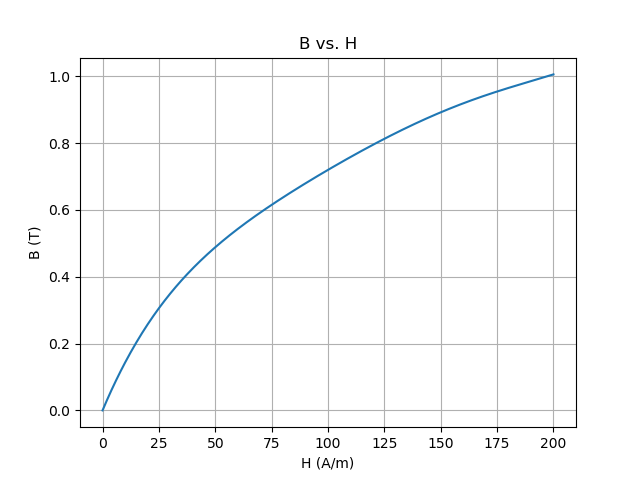
\includegraphics[width=\linewidth]{../data/B_H_first_six}
				\caption{Interpolation of the First Six Data Points}
				\label{bh_first6}
			\end{figure}
		
			From the figure, the interpolation has returned a plot with a \textbf{plausible} result over this range. 
		\subsection{Lagrange Full Domain Interpolation of the Second Six-Point Set}
			Select a second data point set, the Lagrange interpolation returned a polynomial of 
			\begin{align*}
				B(h) = &7.467\times 10^{-19}h^5 - 3.505\times 10^{-14}h^4 \\
					   &+ 5.3\times 10^{-10}h^3 - 2.864\times 10^{-6}h^2 \\
					   &+ 3.804\times 10^{-3}h
			\end{align*}
			whose plot is shown in Figure \ref{bh_second6}. 
			\begin{figure}[!h]
				\centering
				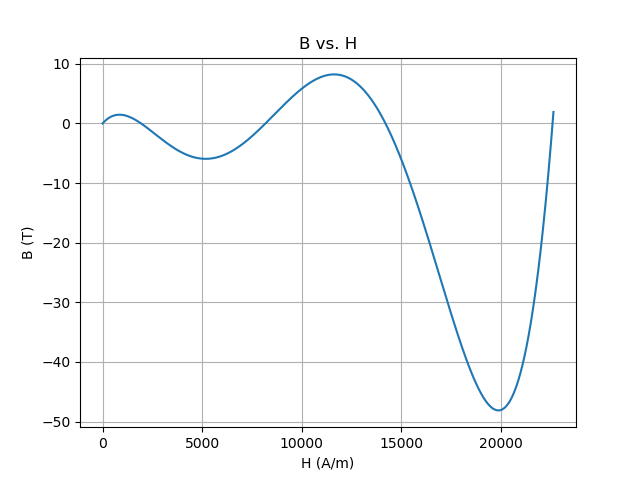
\includegraphics[width=\linewidth]{../data/B_H_second_six}
				\caption{Interpolation of the Second Six Data Points}
				\label{bh_second6}
			\end{figure}
			
			From this plot, we can see that the interpolation using the second set of data points is \textbf{not plausible} as the graph fluctuates violently as the value of $B$ goes to negative at some ranges. 		
		
		\subsection{Cubit Hermite Polynomial Interpolation}
			
		\subsection{Nonlinear Equation of the Magnetic Circuit}
			Consider the magnetic circuit shown in Figure \ref{mag_circuit}. 
			\begin{figure}[!h]
				\centering
				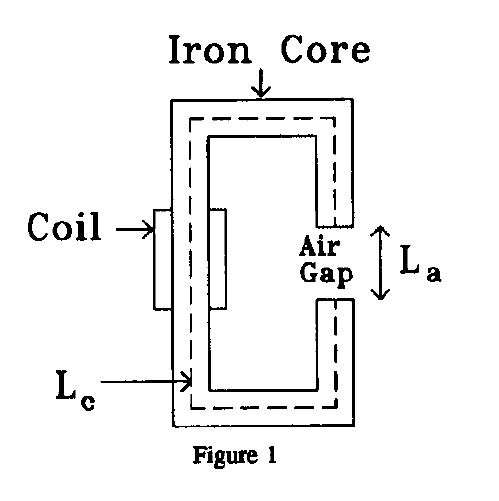
\includegraphics[width=0.8\linewidth]{mag_circuit}
				\caption{The Magnetic Circuit Discussed About}
				\label{mag_circuit}
			\end{figure}
		
			The Magnetomotive force (MMF) can be calculated by Equation \ref{mmf},
			\begin{equation}
				M = (R_g + R_c)\psi
				\label{mmf}
			\end{equation}
			where $R_g$ and $R_c$ are the reluctance of the air gap and the coil, respectively. Plug in the variables from the problem, we can transform Equation \ref{mmf} to the equation as follows:
			\begin{align*}
				M &= (\frac{l_g}{\mu_0A} + \frac{l_c}{\mu A})\psi \\
				NI &= (\frac{l_g}{\mu_0 A} + \frac{l_cH(\psi)}{AB})\psi \\
				NI &= (\frac{l_g}{\mu_0 A} + \frac{l_cH(\psi)}{\psi})\psi
			\end{align*}
			
			Simplify the equation by bringing $NI$ to the right of the equation, and the equation will be the final formula of $f(\psi)$, as is shown in Equation
			\begin{equation}
				f(\psi) = \frac{l_g \psi}{\mu_0 A} + l_cH(\psi) - NI = 0
			\end{equation}
			
			Plug in the numbers, we can finalize the equation by calculating all the coefficients of the polynomial, shown in Equation \ref{final_mmf}.
			\begin{equation}
				f(\psi) = 3.979\times 10^{7}\psi + 0.3H(\psi) - 8000
				\label{final_mmf}
			\end{equation}
	\newpage
	\onecolumn
	\begin{appendices}
		
		\section{Code Listings} \label{appendix:code}
		
		\setminted{linenos,breaklines,fontsize=\footnotesize}
		
		\begin{center}
			\captionof{listing}{Polynomials Implementation (\texttt{polynomial.py}).}
			\inputminted{python}{../polynomial.py}
			\label{lst:poly}
		\end{center}
		\begin{center}
			\captionof{listing}{Lagrange Interpolation Implementation (\texttt{interpolation.py}).}
			\inputminted{python}{../interpolation.py}
			\label{lst:interp}
		\end{center}
	\end{appendices}
\end{document}